\documentclass{article}
\usepackage[utf8]{inputenc}
\usepackage{graphicx}
\usepackage{hyperref}
\usepackage{MnSymbol}

\title{Algoritmo di Ford Fulkerson}
\author{Rosario Cannavò }
\date{Gennaio 2021}

\begin{document}

\maketitle

\section{Introduzione}
\section{Metodo di Ford Fulkerson}
\subsection{Reti residue}
\subsection{Cammini aumentanti}
\subsection{Tagli delle reti di flusso}
\subsection{Algoritmo di base di Ford-Fulkerson}
\subsection{Complessità}
\section{Implementazione}
\subsection{Algoritmo di Edmonds-Karp}
\subsection{Complessità algoritmo di Edmonds-Karp}
\subsection{Struttura Dati}
\subsection{Procedura di Edmonds-Karp}
\subsection{Casi limite}
\subsection{Considerazioni finali}
\subsection{Diagramma UML}


\newpage
\begin{flushleft}
\huge \textbf{1. Introduzione}
\newline
\newline
\normalsize
In informatica, l'algoritmo di Ford-Fulkerson permette di calcolare il flusso massimo tra due nodi di un grafo. Il nome deriva dai suoi due ideatori, Lester Randolph Ford e Delbert Ray Fulkerson. In questo report sarà trattato l'algoritmo e tutti i concetti ad esso legati; sarà, inoltre, trattata l'implementazione del metodo tramite l'algoritmo di Edmonds-Karp.
\newline
Dato un grafo che rappresenta una rete di flusso, in cui ogni arco ha una capacità, e dati due vertici, sorgente $s$ e pozzo $t$, lo scopo è trovare il flusso massimo possibile da $s$ a $t$ rispettando i seguenti vincoli:
\begin{enumerate} 
\item Il flusso su un arco non deve eccedere la capacità dell'arco stesso; 
\item I flussi in entrata e in uscita sono uguali per ogni vertice, eccetto $s$ e $t$.
\end{enumerate}
Per comodità supponiamo che ogni vertice giaccia su qualche cammino dalla sorgente al pozzo e che, dunque, il grafo sia connesso, in quanto ogni vertice diverso dalla sorgente ha almeno un arco entrante.
\end{flushleft}
\begin{figure}[h!]
\begin{center}
  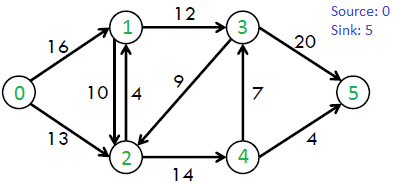
\includegraphics[width=8cm]{ciao.png}\\
\end{center}
\end{figure}
\begin{flushleft}
\normalsize 
La seguente è una semplice idea per l'implementazione dell'algoritmo di Ford-Fulkerson: 
\begin{enumerate} 
\item Il flusso massimo è impostato a 0 all'inizio dell'esecuzione;
\item Fino a quando esiste un cammino aumentante dalla sorgente al pozzo, aggiunge questo percorso al flusso massimo;
\item ritorna il flusso massimo
\end{enumerate}

Prima di dare la spiegazione dell'algoritmo di Ford-Fulkerson e la sua implementazione tramite la strategia di Edmonds-Karp, sarà fornita al lettore una breve introduzione ai concetti di "rete residua", "cammino aumentante" e "flusso massimo".
\end{flushleft}

\newpage
\begin{flushleft}
\huge \textbf{2. Metodo di Ford Fulkerson}
\newline
\newline
\normalsize


Il metodo di Ford-Fulkerson aumenta in modo iterativo il valore del flusso. Iniziamo con $f(u,v) = 0$ per ogni $u,v \in V$, assegnando al flusso iniziale un cammino aumentante in una rete residua associata a $G_f$. Una volta che conosciamo gli archi di un cammino aumentante in $G_f$, possiamo facilmente identificare degli archi specifici in $G_f$, dei quali possiamo modificare il flusso, in modo tale da aumentarne il valore. Sebbene ogni iterazione del metodo di Ford-Fulkerson ne faccia aumentare il valore, vedremo che il flusso in un particolare arco di $G_f$ può sia aumentare che diminuire: una sua diminuzione potrebbe essere necessaria per consentire ad un algoritmo di inviare più flusso dalla sorgente al pozzo.
\newline
Aumentiamo ripetutamente il flusso finchè nella rete residua non ci saranno altri cammini aumentanti. Il \textbf{teorema del flusso massimo} ci garantirà che questo processo genera un flusso massimo.
\end{flushleft}
\begin{flushleft}
FORD-FULKERSON(G,s,t)
\begin{enumerate} 
\item inizializza il flusso $f$ a 0
\item \textbf{while} esiste un cammino aumentante $p$ nella rete residua $G$ aumenta il flusso $f$ lungo $p$
\item \textbf{return} $f$
\end{enumerate}
\end{flushleft}

\hfill
\begin{flushleft}
\begin{Large} \textbf{2.1 Reti residue} \end{Large}
\newline
\newline
Data una rete di flusso $G$ e un flusso $f$, la rete residua $G_f$ è composta da archi con capacità che rappresentano come possiamo modificare il flusso negli archi di $G$. Un arco della rete di flusso può accettare una quantità di flusso aggiuntivo pari alla capacità dell'arco meno il flusso su tale arco. Se tale valore è positivo, inseriamo questo arco in $G_f$ con una \textbf{capacità residua} pari a $c_f(u,v) = c(u,v) - f(u,v)$. Gli unici archi di $G$ che si trovano in $G_f$ sono quelli che possono accettare più flusso. Gli archi $(u,v)$ il cui flusso $p$ è uguale alla loro capacità hanno $c_f(u,v) = 0$; questi archi non si trovano in $G_f$. 
La rete residua $G_f$ può contenere archi che non si trovano in $G$. Quando un algoritmo manipola il flusso, con l'obiettivo di aumentare il flusso totale, potrebbe essere necessario ridurre il flusso di un particolare arco. Per rappresentare una possibile riduzione di un flusso positivo $f(u,v)$ in un arco $G$, poniamo un arco che può accettare un flusso nella direzione opposta a $(u,v)$, che al più può annullare il flusso in $(u,v)$. Questi archi opposti nella rete residua consentono a un algoritmo di inviare un flusso opposto a quello che aveva già inviato in un arco. Inviare un flusso opposto equivale a "ridurre" il flusso nell'arco, che è un'operazione necessaria in molti algoritmi.
\newline
Formalmente, supponiamo di avere una rete di flusso $G = (V,E)$ con una sorgente $s$ e un pozzo $t$. Sia $f$ un flusso in $G$; consideriamo una coppia di vertici $u,v \in V$. definiamo \textbf{capacità residua} $c_f(u,v)$ in questo modo: 
\newline
\end{flushleft} 

\begin{center}
\[c_f(u, v) =\left\{
  \begin{array}{lr}
    c(u,v) - f(u, v) & \mbox{se } (u, v) \in E\\
    f(v, u) & \mbox{se } (v, u) \in E\\
    0 & \mbox{altrimenti}
  \end{array}
\right.
\]
\newline
\end{center}
\begin{flushleft}
Poiché l'ipotesi $(u,v) \in E$ implica che $(v,u) \notin E$, un solo caso del sistema può essere applicato a ciascuna coppia di vertici.
\newline
Data una rete di flusso $G = (V, E)$ con flusso $f$, la \textbf{rete residua} di $G$ indotta da $f$ è $G_f = (V, E_f)$, dove:
\newline
\newline
$E_f = \{(u,v) \in V$ x $V: c_f(u,v) > 0\}$
\newline
\newline
Ovvero, ogni arco della rete residua o \textbf{arco residuo}, può ammettere un flusso che è maggiore di 0.
\newline
Gli archi in $E_f$ o sono archi di $E$ o sono i loro opposti, quindi: $|E_f \leq 2|E|$.
\newline
\newline
La rete residua $G_f$ è simile a una rete di flusso ma non soddisfa la nostra definizione di rete di flusso, perché può contenere sia l'arco $(u,v)$ che il suo opposto $(v,u)$. A parte questo, una rete residua ha le stesse capacità di una rete di flusso e possiamo definire un flusso nella rete residua come quello che soddisfa nella definizione di flusso ma rispetto alle capacità $c_f$ nella rete $G_f$.
\newline
Un flusso in una rete residua rappresenta una guida per aggiungere flusso alla rete originale. Se $f$ è un flusso in $G$ e $f'$ è un flusso nella corrispondente rete residua $G_f$, definiamo:
\newline
$f \uparrow f'$, l'\textbf{aumento} di $f'$ del flusso $f$, come funzione da $V$ x $V$ a $R$ in questo modo:
\newline
\newline
\begin{center}
\[f\uparrow f'(u, v) =\left\{
  \begin{array}{lr}
    f(u, v) + f'(u, v) - f'(v,u) & \mbox{se } (u, v) \in E\\
    0 & \mbox{negli altri casi } 
  \end{array}
\right.
\]
\newline
\end{center}
Il concetto che sta alla base di questa definizione deriva dalla definizione di rete residua. Noi aumentiamo il flusso in $(u, v)$ di $f'(u, v)$, ma lo riduciamo di $f'(v, u)$ perchè immettere un flusso nell'arco opposto della rete residua significa diminuire il flusso nella rete originale. L'immissione di flusso nell'arco opposto della rete residua è detto anche \textbf{cancellazione}.
\end{flushleft}

\hfill
\begin{flushleft}
\begin{Large} \textbf{2.2 Cammini aumentanti} \end{Large}
\newline
\newline
Data una rete di flusso $G = (V, E)$ con flusso $f$, un \textbf{cammino aumentante} $p$ è un cammino semplice da $s$ a $t$ nella rete residua $G_f$. Per definizione di rete residua, possiamo aumentare il flusso di un arco $(u, v)$ in un cammino aumentante fino a $c_f(u, v)$, senza violare il vincolo sulla capacità qualunque sia l'arco $(u, v)$ o $(v, u)$ che si trovi nella rete di flusso originale $G$.
\newline
La quantità massima di cui può crescere il flusso in ogni arco di un cammino aumentante $p$ è detta \textbf{capacità residua} di $p$ ed è espressa da:
\newline
\newline
$c_f(p) = min \{c_f(u, v): (u, v) \in p \}$
\end{flushleft}
\begin{figure}[ht!]
\begin{center}
  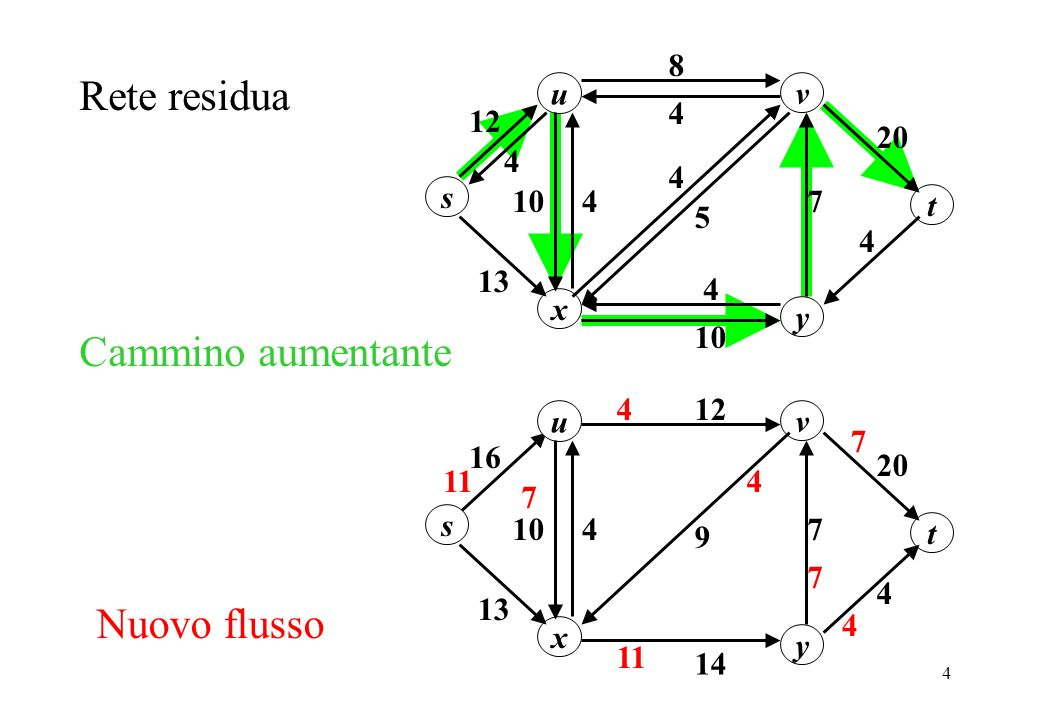
\includegraphics[width=8cm]{rete.jpg}\\
\end{center}
\end{figure}
\hfill
\begin{flushleft}
\begin{Large} \textbf{2.3 Tagli delle reti di flusso} \end{Large}
\newline
\newline
Il metodo di Ford-Fulkerson incrementa ripetutamente il flusso lungo i cammini aumentanti, finchè non viene trovato un flusso massimo. Come facciamo a sapere di aver trovato un flusso massimo quando l'algoritmo termina? Il \textbf{teorema del flusso massimo}, ci dice che un flusso è massimo se e solo se la sua rete residua non contiene cammini aumentanti.Per enunciare questo teorema è necessario introdurre il concetto di taglio di una rete di flusso.
\newline
Un \textbf{taglio} $(S, T)$ della rete di flusso $G = (V, E)$ è una partizione di $V$ in $S$ e $T = V - S$ tale che $s \in S$ e $t \in T$.
\newline
Se $f$ è un flusso, allora il \textbf{flusso netto} $f(S, T)$ attraverso il taglio $(S, T)$ è definito come:
\newline
\newline
\begin{center}
$f(S, T) =  \sum\limits_{u \in s} \sum\limits_{v \in T} f(u,v) -  \sum\limits_{u \in s} \sum\limits_{v \in T} f(v,u)$
\newline
\end{center}
La \textbf{capacità} del taglio $(S,T)$ è:
\newline
\newline
\begin{center}
$c(S, T) =  \sum\limits_{u \in s} \sum\limits_{v \in T} c(u,v)$
\newline
\end{center}
Un \textbf{taglio minimo} di una rete è un taglio la cui capacità è minima rispetto a tutti i tagli della rete.
\newline
\newline
\begin{large}\textbf{Teorema del flusso massimo}\end{large}
\newline
\newline
Se $f$ è un flusso in una rete di flusso $G = (V, E)$ con sorgente $s$ e pozzo $t$, allora le seguenti condizioni sono equivalenti:
\begin{enumerate} 
\item $f$ è un \textbf{flusso massimo} in $G$;
\item La \textbf{rete residua} $G_f$ non contiene \textbf{cammini aumentanti};
\item $|f| = c(S, T)$ per qualche taglio $(S, T)$ di $G$,

\end{enumerate}
\end{flushleft}
\hfill
\begin{flushleft}
\begin{Large} \textbf{2.4 Algoritmo di base di Ford-Fulkerson} \end{Large}
\newline
\newline
In ogni iterazione del metodo di Ford-Fulkerson, troviamo qualche cammino aumentante $p$ e utilizziamo $p$ per modificare il flusso $f$. Dunque, sostituiamo $f$ con $f\uparrow f_p$, ottenendo un nuovo flusso il cui valore è $|f| + |f_p|$. La seguente implementazione del metodo calcola il flusso $(u, v).f$ per ogni arco $(u, v) \in E$. Se $(u, v) \notin E$ assumiamo implicitamente che $(u, v).f = 0$. Supponiamo inoltre che le capacità $c(u, v)$ vengano fornite con la rete di flusso e che $c(u, v) = 0$ se $(u, v) \notin E$.

\begin{flushleft}
FORD-FULKERSON(G,s,t)
\begin{enumerate} 
\item \textbf{for} ogni arco $(u, v) \in G.E$
\item \hspace{10pt} $(u, v).f = 0$
\item \textbf{while} esiste un cammino $p$ da $s$ a $t$ nella rete residua $G_f$
\item \hspace{10pt} $c_f(p) = min\{c_f(u, v): (u, v) \in p \}$
\item \hspace{10pt} \textbf{for} ogni arco $(u, v)$ in $p$
\item \hspace{20pt} \textbf{if}$(u, v) \in E$
\item \hspace{30pt} $(u, v).f = (u,v).f + c_f(p)$
\item \hspace{20pt} \textbf{else} $(u, v).f = (v, u).f - c_f(p)$
\end{enumerate}
\end{flushleft}
Le righe 1-2 inizializzano il flusso $f$ a 0. Il ciclo \textbf{while} delle righe 3-8 trova ripetutamente un cammino aumentante $p$ in $G_f$ e incrementa il flusso $f$ lungo $p$ della capacità residua $c_f(p)$. Ogni arco residuo nel cammino $p$ può essere un arco della rete originale o l'opposto di un arco della rete originale. Le righe 6-8 aggiornano appropriatamente il flusso in ciascun caso, sommando il flusso quando l'arco residuo è un arco originale e sottraendo il flusso nell'altro caso. Quando non esistono più cammini aumentanti, il flusso $f$ è un \textbf{flusso massimo}.
\newline
\newline
\begin{large} \textbf{Osservazione} \end{large}
\newline
\newline
Dal teorema del flusso massimo/taglio minimo segue che se esiste un flusso massimo, allora:
\newline
\newline
\begin{center}
$\max\limits_{f flusso in G} |f|  = \min\limits_{(S, T) taglio in G} c(S, T)$
\newline
\end{center}
\end{flushleft}

\hfill
\begin{flushleft}
\begin{Large} \textbf{2.5 Complessità} \end{Large}
\newline
\newline
Il tempo di esecuzione della procedura di Ford-Fulkerson dipende da come viene determinato il cammino aumentante $p$ alla linea 4.
\newline
Se questa scelta viene fatta male la procedura \textbf{può anche non terminare}.
\newline
Se si suppone che tutte le capacità della rete siano dei valori interi, allora una semplice implementazione della procedura di Ford-Fulkerson ha un tempo di esecuzione \textbf{$O(E|f*|)$} dove $f*$ è il flusso massimo trovato dall'algoritmo, infatti:
\newline
\begin{itemize}
    \item il ciclo \textbf{for} 1-3 richiede tempo $O(E)$;
    \item il ciclo \textbf{while} 3-8 viene eseguito al massimo $|f*|$ volte, perchè il valore del flusso aumenta almeno di una unità ad ogni iterazione; inoltre, ad ogni iterazione, un cammino aumentante può essere calcolato in tempo $O(E)$, mediante una visita della \textbf{rete residua} $G_f$ da $s$ fino a trovare $t$.
\end{itemize}
\end{flushleft}


\newpage
\begin{flushleft}
\huge \textbf{3. Implementazione}
\newline
\newline
\normalsize
\hfill
\newline
\begin{Large} \textbf{3.1 Algoritmo di Edmonds-Karp} \end{Large}
\newline
\newline
Il limite superiore per il tempo di esecuzione della procedura Ford-Fulkerson può essere migliorato se si realizza il calcolo del cammino aumentante $p$ tramite una \textbf{visita in ampiezza} (BFS), cioè se il cammino aumentante selezionato è un \textbf{cammino minimo} da $s$ a $t$ nella rete residua, dove ogni arco ha distanza unitaria.
\newline
Il metodo di Ford-Fulkerson così modificato prende il nome di \textbf{Algoritmo di Edmonds-Karp}.
Allegata al report, sarà fornita l'implementazione del metodo di Ford-Fulkerson tramite algoritmo di Edmonds-Karp in linguaggio C++.
\end{flushleft}
\begin{flushleft}
\hfill
\newline
\begin{Large} \textbf{3.2 Complessità algoritmo di Edmonds-Karp}\end{Large}
\newline
\newline
L'algoritmo di Edmonds-Karp abbassa la complessità totale a $O(VE^2)$ quando il grafo viene rappresentato tramite \textbf{liste di adiacenza}.
\newline
Nell'implementazione fornita, il grafo verrà rappresentato tramite \textbf{matrici di adiacenza} per semplicità; questa tipologia di rappresentazione porta la complessità a $O(VE^3)$.
\newline
Dai teoremi sulle reti di flusso per il metodo di Edmonds-Karp (Prof. Cantone Domenico, \textit{Appunti sulle reti di flusso}, A.A. 2017/2018), possiamo dimostrare che la complessità dell'algoritmo di Edmonds-Karp è al massimo $O(VE^2)$.
\newline
\newline
 \textbf{Dimostrazione}
\newline 
\newline
Dal teorema sulle reti residue citato, segue che il numero di incrementi di flusso è al più $|V| \cdot |E|$. Inoltre, il costo computazionale di ciascun incremento è $O(E)$ (effettuando una visita in ampiezza dalla sorgente $s$
 nella rete residua sino a trovare il pozzo $t$). Pertanto, segue la tesi.
\end{flushleft}

\begin{flushleft}
\hfill
\newline
\begin{Large} \textbf{3.3 Struttura Dati}\end{Large}
\newline
\newline
La struttura adoperata per l'esecuzione dell'algoritmo è un grafo orientato che prende il nome di \textbf{rete di flusso}. Nella rete di flusso $G = (V, E)$, ogni arco $(u, v) \in E$ ha una \textbf{capacità} non negativa $c(u, v)\geq 0$. Inoltre, se esiste un arco $(u, v) \in E$, non può esserne presente uno opposto $(v, u)$. Per semplicità, se un arco non appartiene ad E la sua capacità è uguale a zero e non sono ammessi cappi.
\newline
Nella rete si distinguono due nodi chiamati \textbf{sorgente} $s$ e \textbf{pozzo} $t$.
\newline
Per comodità supponiamo che ogni nodo giaccia su un cammino dalla sorgente al pozzo, ovvero, $\forall$  $v \in V$  $\exists$ un cammino $s \leadsto v \leadsto t$. Si osserva dunque che il grafo è \textbf{connesso} poichè ogni vertice diverso da s ha almeno un arco entrante.
\newline
\newline
Il grafo presente nella codifica è una classe grafo che sfrutta le matrici di adiacenza e coinvolge le classiche operazione di manipolazione su archi e nodi. Inoltre all'interno del grafo sono presenti la funzione BFS che esegue una ricerca in ampiezza e la funzione "Ford-Fulkerson" che implementa il metodo di Ford-Fulkerson e ritorna il flusso massimo del grafo costruito in input. 
\newline
\newline

\begin{Large}\textbf{3.4 Procedura di Edmonds-Karp}\end{Large}
\newline
\newline
Come abbiamo osservato,il grafo residuo di una rete di flusso è un grafo che indica il flusso aggiuntivo possibile. Se esiste un percorso dalla sorgente al pozzo nel grafo residuo, è possibile aggiungere il flusso parziale a quello massimo. Ogni arco di un grafo residuo ha un valore chiamato capacità residua che è uguale alla capacità originale dell'arco meno il flusso di corrente. La capacità residua è fondamentalmente la capacità attuale dell'arco.
\newline
Possiamo inizializzare il grafo residuo come il grafo originale poiché non c'è flusso iniziale e la capacità residua inizialmente è uguale alla capacità originale. Per trovare un cammino aumentante, possiamo usare una BFS nel grafo residuo. Utilizzando la BFS, è possibile scoprire se esiste un percorso dalla sorgente al pozzo (questo percorso sarà sempre minimo). Inoltre, la BFS costruisce un array parent[]: utilizzando l'array parent[], attraversiamo il percorso trovato e ne ricaviamo la capacità residua minima. Successivamente aggiungeremo il flusso del percorso trovato al flusso complessivo.
Ad ogni ciclo è importante aggiornare le capacità residue nel grafo residuo per garantire il funzionamento dell'algoritmo.
\newline
\newline
\newline
\begin{Large}\textbf{3.5 Casi limite}\end{Large}
\newline
\newline
Nella codifica dell'algoritmo sono presenti anche dei controlli che permettono la gestione di eccezioni e di alcuni casi limite. Uno tra questi è la presenza di una rete di flusso sprovvista di nodi, dunque un grafo in cui $|E| = 0$. Per poter gestire questo caso, è sufficiente effettuare un controllo a livello di struttura, andando a verificare prima dell'esecuzione dell'algoritmo in se, la cardinalità del grafo istanziato sul quale si vuole richiamare la procedura: se essa è uguale a zero, l'algoritmo non verrà eseguito e restituirà il valore di check "-1".
\newline
\vspace{100pt}
\newline

\begin{Large}\textbf{3.6 Considerazioni finali}\end{Large}
\newline

Per quanto riguarda l'approccio puramente implementativo, la rete di flusso è stata definita tramite matrice di adiacenza esclusivamente per semplificare le operazioni sul grafo, andando, però, a discapito della complessità, aumentandola di un ordine di n. Dal punto di vista della complessità spaziale, si è preferito mantenere una sola matrice, rappresentante sia l'adiacenza dei nodi che il peso di questi ultimi, presupponendo come citato in precedenza che gli archi assenti abbiano capacità zero.
\newline
\newline
Nel grafo sono presenti solo poche operazioni base necessarie al funzionamento dell'algoritmo, in quanto la struttura non è il cuore del progetto ma viene utilizzata esclusivamente come supporto per l'algoritmo preso in considerazione.
Per il motivo prima citato, è stato, dunque, deciso di implementare una singola classe contenente attributi e metodi necessari, evitando così di aumentare il contenuto con argomenti poco attinenti e  concentrando tutte le risorse sull'algoritmo stesso.
\newline
Per quanto riguarda la procedura, è stato preferito l'approccio di Edmonds-Karp in quanto è uno dei metodi più efficienti conosciuti tra le varie implementazioni dell'algoritmo di Ford-Fulkerson; inoltre, è stato preferito quest'approccio perchè esso sfrutta strumenti semplici già noti come la visita in ampiezza e il concetto di array dei predecessori. 
\end{flushleft}
\newpage
\begin{flushleft}
\begin{Large}\textbf{3.7 Diagramma UML}\end{Large}
\newline
\normalsize
\begin{figure}[ht!]
\begin{center}
  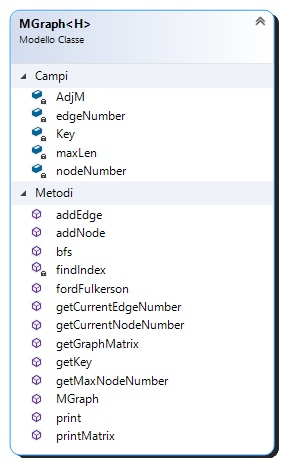
\includegraphics[width=7.5cm]{ClassDiagram.jpg}\\
\end{center}
\end{figure}
\end{flushleft}
\hfill{}
\newpage
\begin{flushleft}
Il \textbf{codice} relativo all'implementazione dell'algoritmo citata nel report è reperibile presso: \underline{\url{https://github.com/rosariocannavo/Ford-Fulkerson}}.
\end{flushleft}
\vspace{0pt}
\begin{flushleft}
\begin{large}\textbf{Riferimenti bibliografici}\end{large}
\newline
\newline
\textit{Prof. Cantone Domenico, "Appunti sul metodo di Ford Fulkerson" A.A. 2017/18.}
\newline
\newline
\textit{Thomas H. Cormen, Charles E. Leiserson, Ronald L. Rivest, Clifford Stein, "Introduction to Algorithms, Third Edition" 2010, McGraw-Hill.  }
\newline
\newline
\textit{"Algoritmo di Ford-Fulkerson", Wikipedia, l'enciclopedia libera.}
\end{flushleft}


\end{document}
